\documentclass[tikz]{standalone}
\usepackage[utf8]{inputenc}
\usetikzlibrary{intersections}

\definecolor{DarkBlue}{rgb}{0.0,0.0,0.6}
\definecolor{DarkRed}{rgb}{0.7,0.2,0.2}

\begin{document}

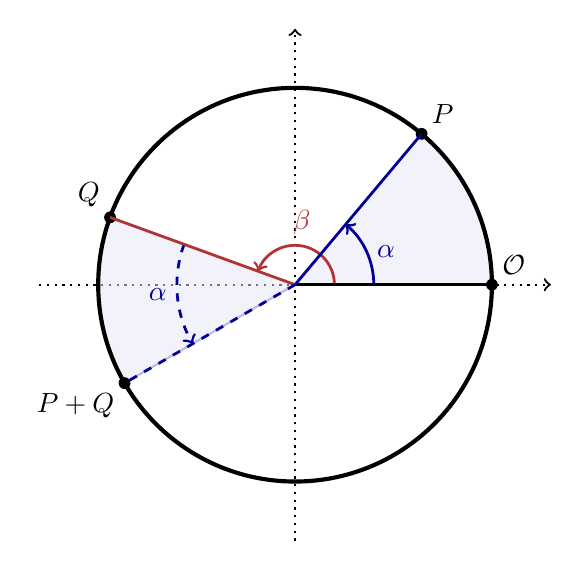
\begin{tikzpicture}[thick,scale=2.5]
\def\ptsize{.03}
\newcount\Pangle
\newcount\Qangle
\newcount\Rangle
\Pangle=50
\Qangle=160
\Rangle=\Pangle
\advance\Rangle by \Qangle
\draw[->,dotted] (-1.3, 0) -- (1.3,0);
\draw[->,dotted] (0,-1.3) -- (0,1.3);
\coordinate[label=above right:$\mathcal{O}$] (inf) at (1,0);
\coordinate[label=above right:$P$] (P) at (\number\Pangle:1);
\coordinate[label=above left:$Q$] (Q) at (\number\Qangle:1);
\coordinate[label=below left:$P+Q$] (R) at (\number\Rangle:1);

\draw[DarkBlue!50,fill=DarkBlue!10,opacity=.5] (0,0) -- (inf) arc (0:\number\Pangle:1) -- cycle;
\draw[DarkBlue!50,fill=DarkBlue!10,opacity=.5] (0,0) -- (Q) arc (\number\Qangle:\number\Rangle:1) -- cycle;

\path[draw,name path=circ,line width=1.5pt] (0,0) circle (1);
\fill (inf) circle (\ptsize);
\fill (P) circle (\ptsize);
\fill (Q) circle (\ptsize);
\fill (R) circle (\ptsize);

\draw[DarkBlue,line width=1pt,->] (.4,0) arc (0:\number\Pangle:.4) node[midway,right] {$\alpha$};
\draw[DarkRed,line width=1pt,->] (.2,0) arc (0:\number\Qangle:.2) node[midway,above] {$\beta$};
\draw[DarkBlue,line width=1pt,->,dashed] (\number\Qangle:.6) arc (\number\Qangle:\number\Rangle:.6) node[midway,left] {$\alpha$};

\draw[line width=1pt] (0,0) -- (inf);
\draw[line width=1pt,DarkBlue] (0,0) -- (P);
\draw[line width=1pt,DarkRed] (0,0) -- (Q);
\draw[line width=1pt,DarkBlue,dashed] (0,0) -- (R);
\end{tikzpicture}

\end{document}